
\section{Introduction}

With recent advances in earthquake ground motion simulation using physics-based methods and hybrid approaches \citep[e.g.,][]{Bielak_2010_GJI, Graves_2010}, verification and validation (V\&V) of synthetics have become increasingly relevant. V\&V imply processing signals in preparation to perform qualitative and quantitative comparisons. We are particularly interested in investigating the effect that different filtering procedures and parameters can have on quantitative validations done using the goodness-of-fit (GOF) method introduced by Anderson (2004). In this method, the degree of similarity between two signals is quantified by means of a set of ten (error) metrics, labeled C1 through C10. These metrics include ground motion characterization parameters commonly used in seismology and earthquake engineering. The quantitative comparisons are projected on a 0?10 scoring scale, where a score of 10 corresponds to a perfect match. When using Anderson?s method, signal pairs are compared by component of motion and at different frequency ranges to weight the contribution of different wavelengths so that low frequencies are given more weight than high frequencies.

The scores of each frequency band, component, and metric are then combined to obtain a final GOF value. \citet{Khoshnevis_2015} found that filtering, in particular, can play a significant role in the output of the GOF scores. Also they showed that the variation of the order of a finite impulse response (FIR) filter has a substantial influence on the GOF scores, especially on those metrics that are strongly time dependent. Therefore, among the metrics considered in the GOF method, the Arias intensity score, and the peak acceleration, velocity and displacement scores are most sensitive; followed by the scores derived from the energy integral, energy duration, Arias duration, cross correlation, response spectra and Fourier spectra; with the latter being the least sensitive of all.

\begin{figure*}
    \centering
    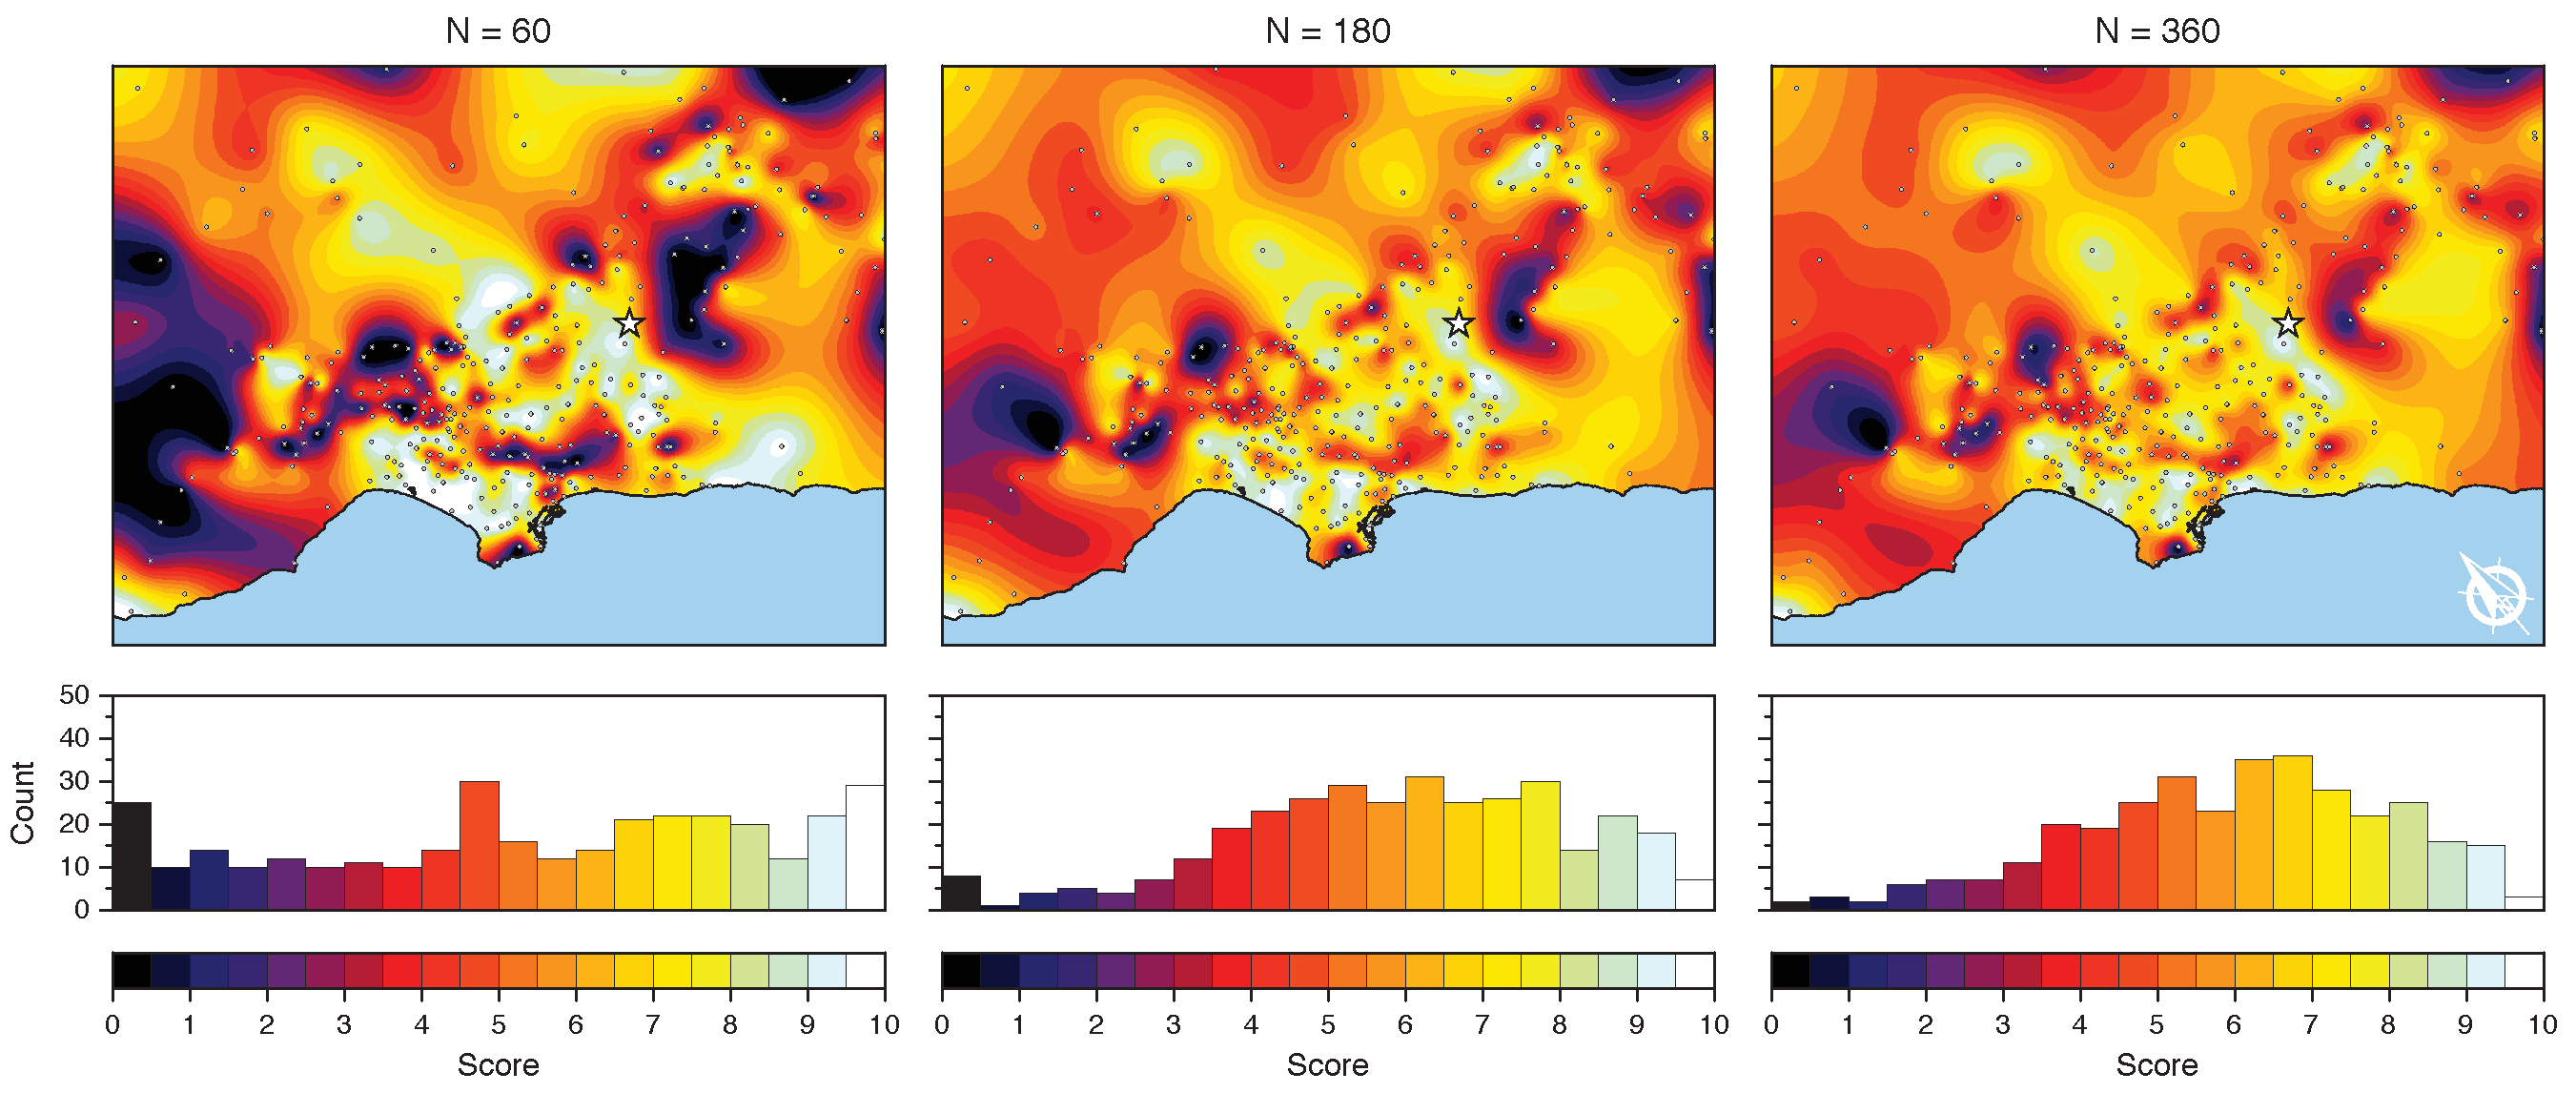
\includegraphics
        [width=\textwidth]
        {figures/pdf/figure1.pdf} 
    \caption{Variation of PGA GOF scores for the case study of the 2008 Mw 5.4 Chino Hills, California, earthquake using FIR Chebyshev filters with order N = 60 (left), 180 (center) and 360 (right). Top frames show contours drawn based on GOF values derived from 336 stations with records used for the comparisons against synthetics from \citet{Taborda_2013_BSSA}. Bottom frames show histogram distributions in the GOF scale introduced by \citet{Anderson_2004}.}
\end{figure*}

\begin{figure}
    \centering
    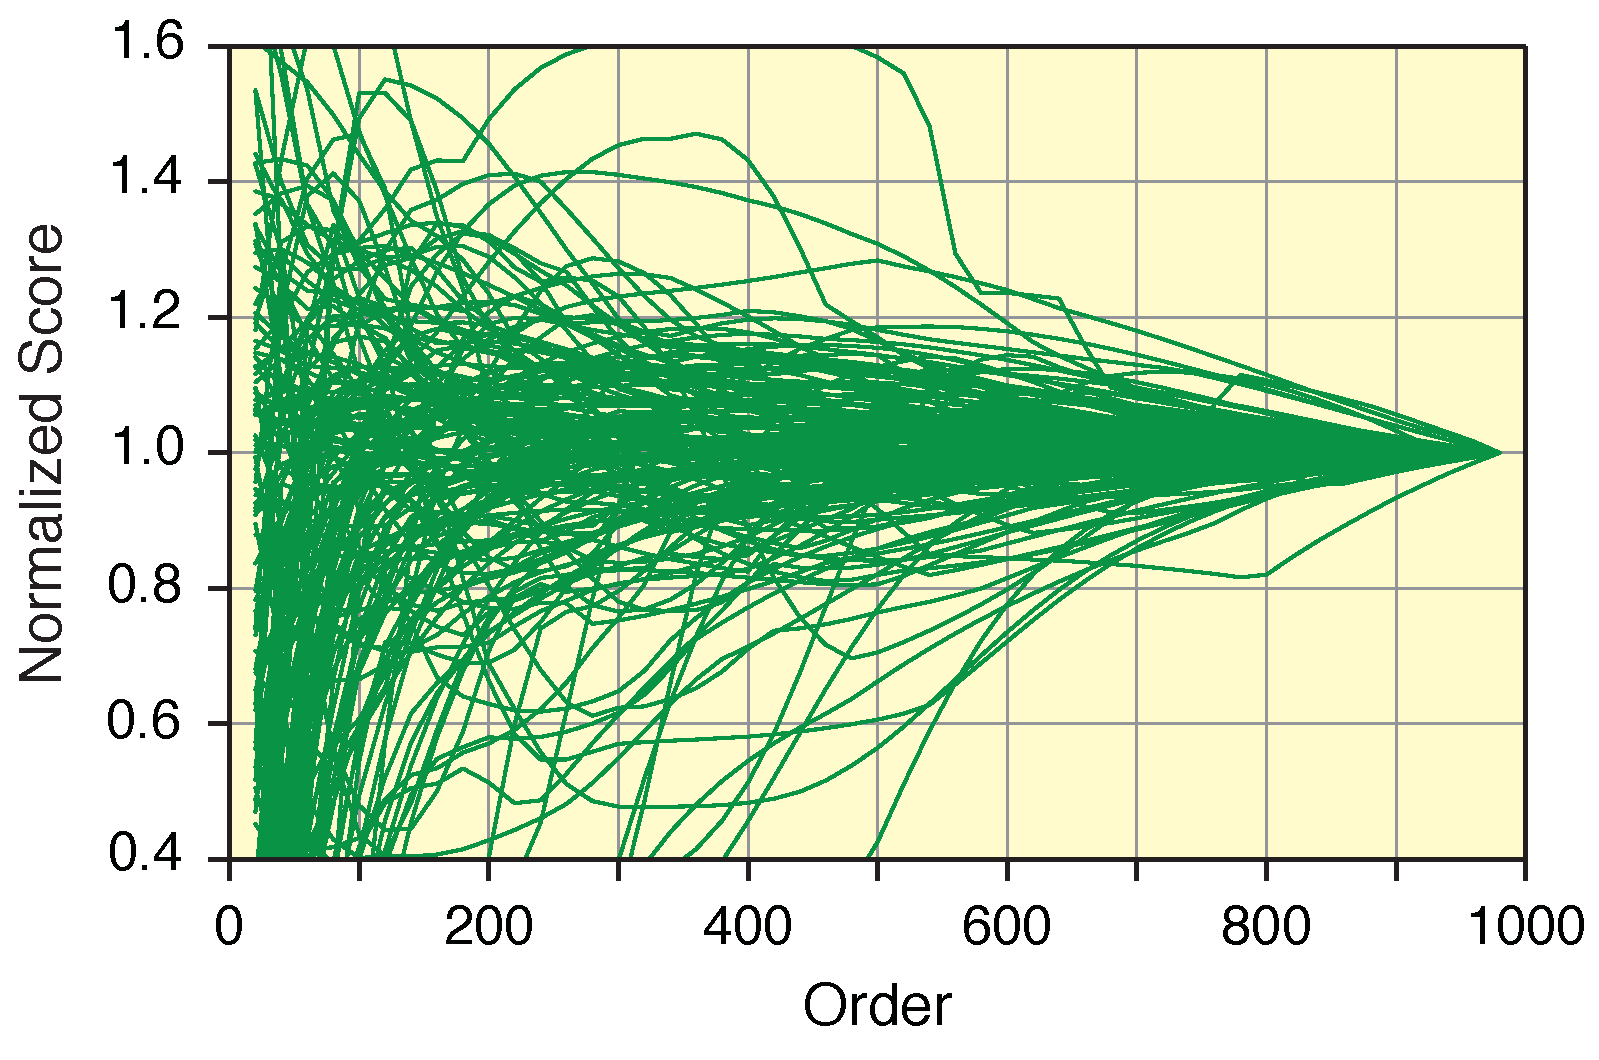
\includegraphics
        [width=\columnwidth]
        {figures/pdf/figure2.pdf} 
    \caption{Variation of PGA GOF scores with increasing order of FIR Chebyshev  filter for the same 336 stations used for the  validation of the Chino Hills earthquake simulation.}
\end{figure}

Figure 2 shows the variation of PGA GOF scores with filter order for the same 336 signal pairs from the Chino Hills simulation. Each score trend is normalized with respect to the value obtained with the highest order. Despite the chosen normalization, the substantial variability over the range of order values suggests that, even for higher order filters, there is not one stable score. Using different types of filters can also be influential on the results. \citet{Khoshnevis2015} implemented a Chebyhsev I infinite impulse response (IIR) filter, instead. As we will explain in greater detail below, IIR filters have sharper cutoffs at the corner frequencies, yet they present ripples in the passband. Figure 3 shows the frequency response of a FIR and an IIR bandpass filter and a comparison of a portion of the Fourier amplitude spectra around the cutoff frequency of a signal filtered using these two type of filters, along with the unfiltered signal. As it can be seen in this figure, the amplitudes of the FIR filtered signal and the original signal are nearly identical within a portion of the passband, but they differ from each other over a wider transition zone than that of the IIR filter.

In turn, the IIR filter does not have a perfect match within the passband, but it exhibits a sharper decay past the cutoff frequency. Arguably, for most applications, these differences are minor and inconsequential. Their effect on GOF scores used for validation may, however, become relevant, especially in the absence of a well-accepted standard. 

\begin{figure}[t]
    \centering
    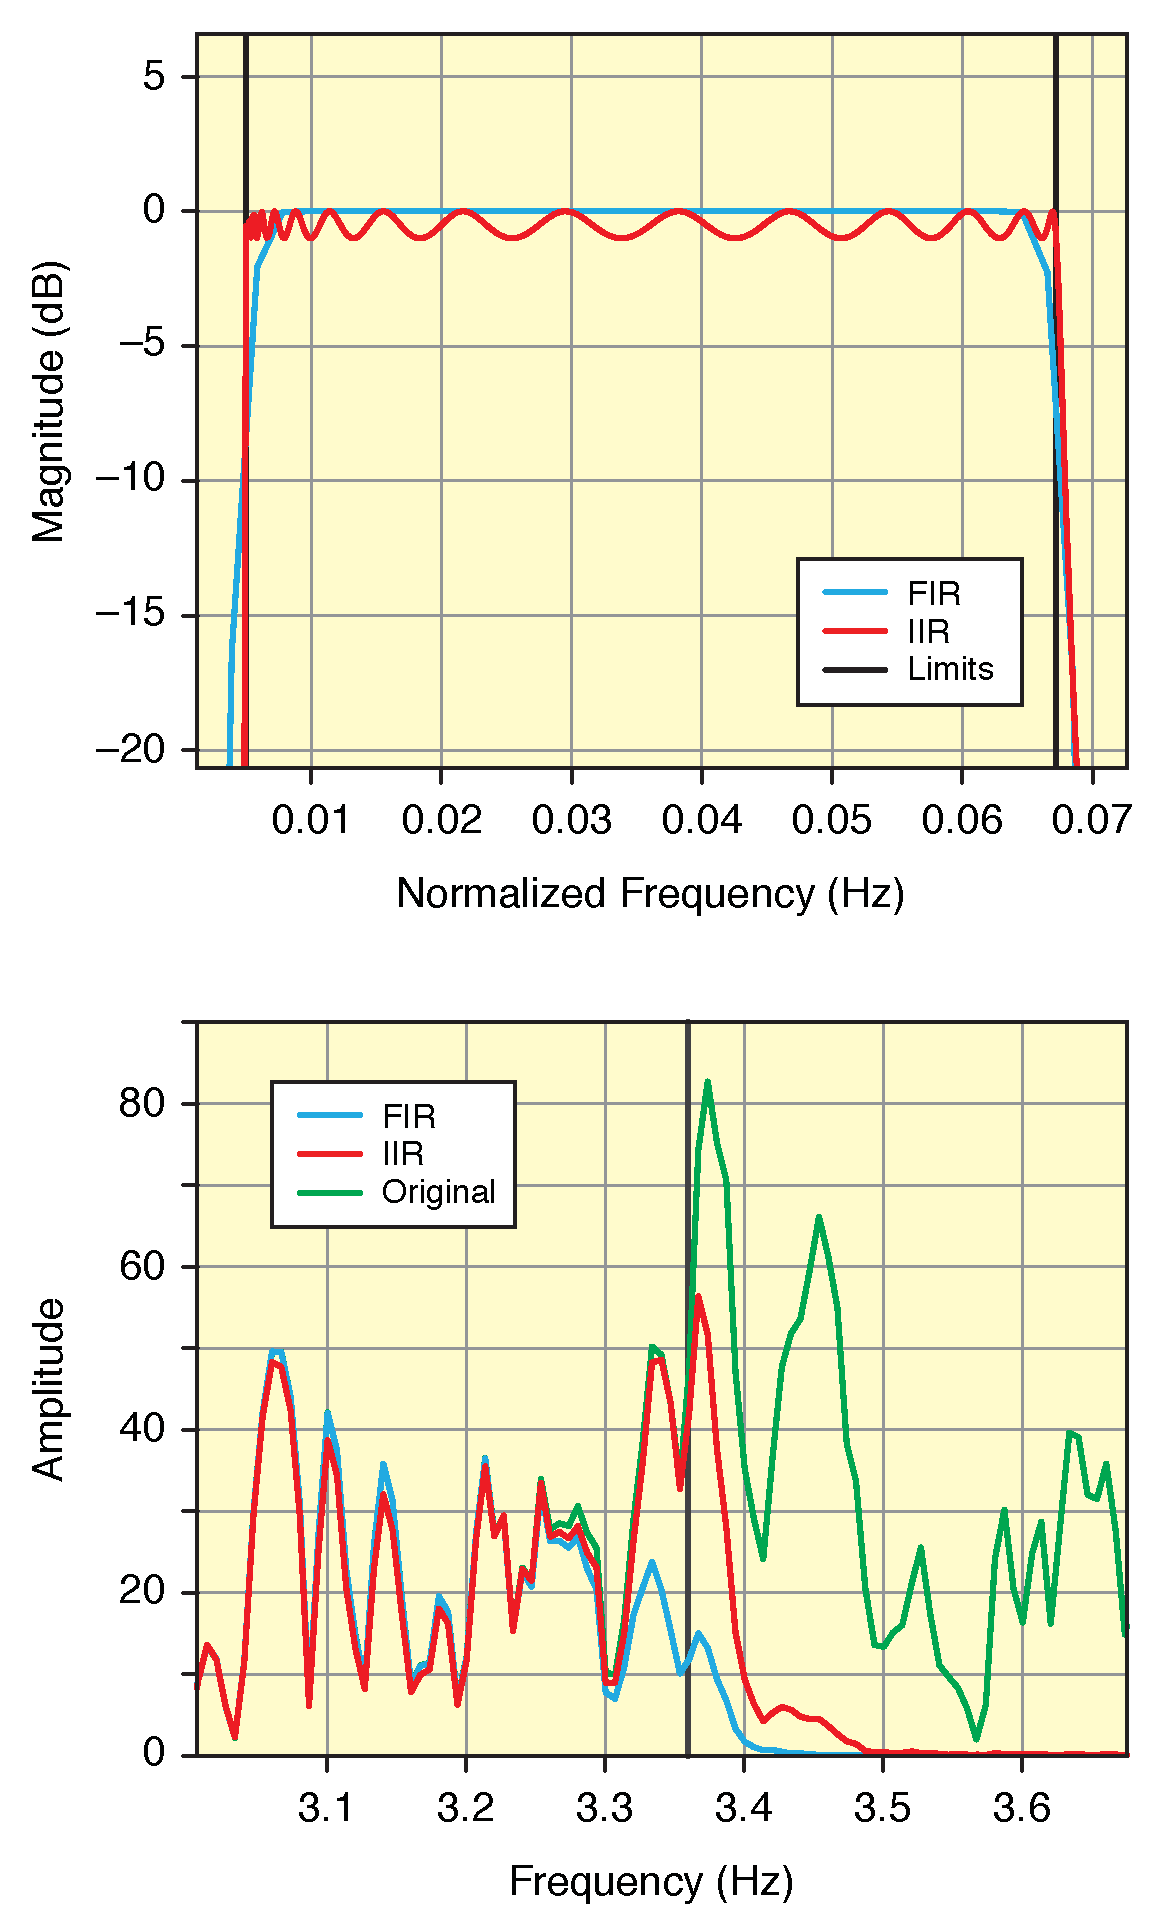
\includegraphics
        [width=\columnwidth]
        {figures/pdf/figure3.pdf} 
    \caption{Comparison between FIR and IIR filters. Top: amplitude response (dB) of the bandpass filters' design in normalized frequency for corner frequencies equal to 0.1 and 0.3 of the maximum frequency. Bottom: detail of a Fourier amplitude spectra around the upper cutoff frequency of a signal filtered with both IIR and FIR filters (the original signal is also included).}
\end{figure}

Moreover, since simulations involve numerous unknowns and assumptions, it is imperative to minimize the additional uncertainties that post-processing of the data may have on the analysis of results. In this paper we seek to contribute to reducing such additional uncertainties by investigating the characteristics of filters used in ground motion signal processing for validation purposes. While it would be difficult to decide on a final ideal filter, it is desirable to define a filter that can be used consistently in validation studies with minor effects on the analysis. Here, we contribute to such an objective. We review the characteristics of the most commonly used FIR and IIR filters, and make initial recommendations on the selection of suitable filter for ground motion simulation validation. Among IIR filters Butterworth filter is more common to use in seismological studies \citep{Ma_2008,Lee_2014,Olsen_2003}. For many of application the filter presents good results. The Butterworth filter is defined based on having uniform sensitivity for wanted frequencies and completely reject unwanted frequencies. Designing filter is trade of between parameters of passband, transition zone, and stopband(i.e. filter order, allowable ripple, min stop band attenuation). Butterworth filter even though completely preserve the passband magnitude and almost completely reject the stop band however it is not successful in transition zone. Even though Butterworth filter designed to have uniform sensitivity of wanted frequency, we can decrease the allowable ripple in elliptic filter to have almost uniform results. However we may not able to decrease the transition zones width in Butterworth filter through commonly used signal processing packages. These transition zones are very important when we are studying very narrow bands. \citet{Oppenheim_1989} suggests using elliptic filter in order to have accurate results in both inside and outside of the band. \citet{Khoshnevis_2015} in a preliminary study shows that elliptic filter gives good results. Elliptic filter can take more input parameter as factors for controlling the filter behavior.   In this paper we are presenting best parameters based on bandwidth to use in filtering process of validation studies. 
